%\documentclass[10pt, english, pdftex]{template/UC3M_document}
 \documentclass[10pt, spanish, pdftex]{template/UC3M_document}

%%%%%%%%%%%%%%%%%%%%%%%%%%%%%%%%%%%%%%%%%%%%%%%%%%%%%%%%
%               UC3M Work report template              %
%           Universidad Carlos III de Madrid           %
%              Author: Aitor Alonso Núñez              %
%              Last update: January 2019               %
%%%%%%%%%%%%%%%%%%%%%%%%%%%%%%%%%%%%%%%%%%%%%%%%%%%%%%%%

%%%%% Preamble %%%%%
\author{Lucía Ruz}         % This is me! You should write here your name (for PDF metadata)
%%%%% About the authors (will be used on title page and header) %%%%%

%%% Indicate the number of authors by uncommenting the right option.
% \authorstwotrue     % 1 or 2 authors
\authorsthreetrue   % 3 authors
%\authorsfourtrue    % 4 authors

%%% Fill with the authors data. You can leave empty keys {} if you need to and also if you provide more info that number of authors indicated it will be ignored.
% If you selected \authorstwotrue or \authorsthreetrue (1 to 3 authors)
\authorsuptothree{Santiago Ramos Sevillano}{NIA 100383401}{Gr. 83}{Iván Valbuena Gálvez}{NIA 100383375}{Gr. 83}{Lucía Ruz Sáez}{NIA 100363940}{Gr. 83}
% If you selected \coauthorsfourtrue (4 authors)
%\authorsfour{Name1 Lastname1}{NIA 100XXXXXX}{Name2 Lastname2}{NIA 100XXXXXX}{Name3 Lastname3}{NIA 100XXXXXX}{Name4 Lastname4}{NIA 100XXXXXX}{Group XX}

%%% If you want to show coauthors email address on the title page, uncomment \emailtrue. Comment it otherwise.
\emailtrue
% You can leave empty keys {} if you need to and also if you provide more info that number of authors indicated or \emailtrue is commented it will be ignored.
\emails{100383401@alumnos.uc3m.es}{100383375@alumnos.uc3m.es}{100363940@alumnos.uc3m.es}{}


%%%%% Basic data about the document (Degree, subject, title, campus, page number custom text) %%%%%
\documentdata{Ingeniería Informática}{Diseño de Sistemas Operativos}{Practica 1: Planificación de procesos}{EPS}{Page }

%%%%% Page style %%%%%
\header
\footer
\pagestyle{fancy}

\begin{document}
%%%%% Page title %%%%%
\titleMain

%%%%% Index %%%%%
\begin{spacing}{0.5}
    % \shipout\null                   % Blank page before index (after title page)
    \hypersetup{linkcolor=black}    % References/links on the index will remain black color
    \tableofcontents        % Index of the document
    \vspace{0.5cm}
    \listoffigures          % Index of pictures
    \vspace{0.5cm}
    \listoftables\newpage           % Index of tables
\end{spacing}


%%%%% DOCUMENT CONTENT %%%%%
\section{Introducción}
A través del presente documento se van a definir los pasos seguidos para el desarrollo de \textbf{tres algoritmos de planificación de hilos en el espacio de usuario}, los cuales se encuentran escritos en el lenguaje de programación C. Estos planificadores han sido creados siguiendo, tanto las pautas dadas en el enunciado de la práctica, como aquellos conocimientos básicos impartidos en la asignatura \textit{Diseño de Sistemas Operativos}.

En primer lugar, es necesario recordar que todos los \textbf{cambios de contexto} en la planificación de procesos de esta práctica se van a realizar en \textbf{espacio de usuario}.

El primer planificador es \textbf{Round-Robin}. El objetivo de esta política es que cada hilo ejecuta un número determinado de ticks definidos en la rodaja, y una vez terminado dicho número de paso al siguiente hilo listo para ejecutar. El documento final donde se encuentra el código de dicho planificador será nombrado como \textbf{\textit{RR.c}}.

Por otro lado, la segunda política ha de ser \textbf{Round-Robin}, para aquellos hilos con prioridad baja, y \textbf{Shortest Job First con prioridades}, para aquellos hilos de prioridad alta. La política Short Job First ejecuta, en primer lugar, aquellos trabajos más cortos frente a aquellos más largos. El documento donde se encuentra dicho fragmento del código se denomina \textbf{\textit{RRS.c}}.

Por último, el último planificador ha de utilizar nuevamente la política \textbf{Round-Robin} para aquellos hilos con prioridad baja, mientras en los hilos de prioridad alta han de utilizar \textbf{Shortest Job First con prioridades}. La diferencia con la segunda implementación se encuentra en que, para este caso, se ha de añadir como funcionalidad un posible \textbf{cambio de contexto voluntario}. En este caso, el documento donde se encuentra dicho fragmento de código se denomina \textbf{\textit{RRSD.c}}.

\section{Diseño usado en el código}
Para el diseño del código se ha analizado el problema inicial, y a continuación se indican las estructuras de datos y funciones implementadas para cada caso en pseudocódigo. 

Es importante destacar que para la realización de nuestros planificadores nos hemos basado en el uso de dos variables globales, \textbf{running} (que ya venía definida en el código base) y \textbf{prev}, que es del mismo tipo que running. La idea es tener siempre un control tanto del hilo que sale de ejecutar (ya sea por fin de rodaja, fin de ejecución, expulsión o bloqueo del mismo) como del hilo que entra a ejecutar. Por lo tanto, \textbf{running} siempre almacenará el hilo al que le toca ejecutar (a excepción de cuando ejecute el hilo \textbf{idle}) y \textbf{prev} el que sale de ejecución, es decir, al realizar un cambio de contexto el hilo que estaba ejecutando \textbf{(running)} se almacenará en \textbf{prev} y \textbf{running} llamará al planificador para obtener el siguiente hilo a ejecutar. Debido a esta decisión de diseño no hemos hecho uso de la función \textbf{\textit{mythread\_gettid}} puesto que ya tenemos un control de los id de los hilos.

Además, es preciso mencionar que en la función \textbf{\textit{mythread\_setpriority}}, al igual que se da unos \textit{remaining\_ticks} a los procesos de prioridad alta se lo hemos dado a los de prioridad baja, evitando casos en los que si el hilo 0 era de baja prioridad y era expulsado por uno de alta prioridad o llamaba a \textit{read\_disk}, su tiempo se acababa y era expulsado. (No obstante haremos pruebas para comprobar que la expulsión de hilos funciona correctamente)

\textbf{Nota}: antes de acceder a cualquiera de las colas generadas, ya sea para encolar o desencolar, se procederá a desactivar las interrupciones de reloj y disco en ese orden. Tras realizar la operación con la cola se reactivará la interrupción de disco y luego la de reloj, en ese orden. Esta medida la hemos realizado para los 3 casos que se proponen, aunque en los dos primeros no se use la interrupción de disco.

Las funciones \textit{mythread\_exit()}, \textit{mythread\_timeout()} y \textit{activator(TCB *next)} son iguales en los códigos de los 3 planificadores, con lo cual, para ahorrar espacio y evitar repetir innecesariamente, hemos decidido ponerlas al principio:

\begin{itemize}
    \item \textbf{mythread\_exit():}
     \vspace{-2mm}
    \begin{itemize}
     \setlength{\itemsep}{-1.5mm}
        \item Estado del proceso que ha terminado = FREE
        \item Liberar espacio asignado al proceso que acaba
        \item Llamada al planificador (scheduler)
        \item Activator (hilo a ejecutar)
    \end{itemize}
    \item \textbf{mythread\_timeout(int tid):}
    \vspace{-2mm}
    \begin{itemize}
     \setlength{\itemsep}{-1.5mm}
        \item Estado del proceso que ha terminado = FREE
        \item Liberar espacio asignado al proceso expulsado
        \item Llamada al planificador (scheduler)
        \item Activator (hilo a ejecutar)
    \end{itemize}
    \item \textbf{activator (TCB *next):}
    \vspace{-2mm}
    \begin{itemize}
     \setlength{\itemsep}{-1.5mm}
        \item Si el proceso anterior ha acabado o ha sido expulsado por timeout (su estado es FREE):
        \vspace{-2mm}
        \begin{itemize}
        \setlength{\itemsep}{-1.5mm}
            \item setcontext (nextContext)
        \end{itemize}
        \item Para el resto de los casos:
        \vspace{-2mm}
        \begin{itemize}
            \setlength{\itemsep}{-1.5mm}
            \item swapcontext (prevContext, nextContext)
        \end{itemize}
    \end{itemize}
\end{itemize}


\subsection{Round Robin}
Una vez analizado el enunciado inicial, para poder implementar el planificador Round-Robin en necesario añadir el campo que contabilice los ticks, es decir, las rodajas de tiempo en el BCP, y también es necesario modificar la interrupción de reloj. Por ello:

\subsubsection{Estructuras de datos}
\vspace{-2mm}
    \begin{itemize}
     \setlength{\itemsep}{-1.5mm}
    \item Ticks en el BCP para poder tener en cuenta las rodajas de tiempo.
    \item Cola de procesos. En este caso se reutilizará la cola ofrecida en el enunciado de la práctica \textit{“t\_queue”}.
\end{itemize}

\subsubsection{Funciones}
\begin{itemize}
 \setlength{\itemsep}{-1.5mm}
    \item \textbf{mythead\_create (void (*fun\_addr)( ), int priority, int seconds)}
    \vspace{-2mm}
    \begin{itemize}
     \setlength{\itemsep}{-1.5mm}
        \item Crea un nuevo proceso 
        \item El número de ticks de su BCP son el máximo por rodaja (BCP. ticks = QUANTUM\_TICKS)
        \item El estado pasa a estar listo (BCP.state = INIT)
        \item Insertar en la cola de procesos
    \end{itemize}
    
    \item \textbf{TCB *scheduler ( )}
    \vspace{-2mm}
    \begin{itemize}
     \setlength{\itemsep}{-1.5mm}
        \item Si no está vacía la lista de listos:
        \vspace{-2mm}
        \begin{itemize}
        \setlength{\itemsep}{-1.5mm}
            \item Desencola el primer proceso y lo guarda 
            \item Devuelve el proceso
        \end{itemize}
    \end{itemize}
    
    \item \textbf{timer\_interrupt ( )}
    \vspace{-2mm}
    \begin{itemize}
     \setlength{\itemsep}{-1.5mm}
        \item Running.ticks -= 1
        \item running.remaining\_ticks -= 1
        \item Si running.remaining\_ticks < 0:
        \vspace{-2mm}
        \begin{itemize}
        \setlength{\itemsep}{-1.5mm}
            \item Entonces el hilo debe acabar por timeout y se llama a dicha función pasando el tid del hilo a expulsar.
        \end{itemize}
        \item Si running.ticks <= 0:
        \vspace{-2mm}
        \begin{itemize}
        \setlength{\itemsep}{-1.5mm}
            \item El estado del hilo que estaba ejecutando pasa a listo para ejecutar.
            \item running.ticks = QUANTUM\_TICKS
            \item Encolar en cola de procesos
            \item prev = hilo ejecutado hasta ahora (running)
            \item Llama al planificador (scheduler)
            \item Si el hilo al que le toca ejecutar es distinto al anterior que ejecutó:
            \vspace{-2mm}
            \begin{itemize}
            \setlength{\itemsep}{-1.5mm}
                \item activator (hilo a ejecutar)
            \end{itemize}
        \end{itemize}
    \end{itemize}
\end{itemize}

\subsection{Round-Robin/ SJF con prioridades}
Para poder implementar el planificador \textit{Round-Robin/SJF} en necesario añadir el campo que contabilice los ticks, es decir, las rodajas de tiempo en el BCP, y también es necesario modificar la interrupción de reloj. Por ello:

\subsubsection{Estructuras de datos}
\vspace{-2mm}
\begin{itemize}
\setlength{\itemsep}{-1.5mm}
    \item Ticks en el BCP: para poder tener en cuenta las rodajas de tiempo.
    \item Cola de procesos: llamada “t\_queue” para albergar los procesos de baja prioridad.
    \item Cola de procesos de alta prioridad: llamada “t\_queue\_high” para albergar los procesos de alta prioridad ordenados de menor a mayor según su duración (remaining\_ticks).
\end{itemize}

\subsubsection{Funciones}
\begin{itemize}
    \item \textbf{mythead\_create (void (*fun\_addr)( ), int priority, int seconds):}
    \vspace{-2mm}
    \begin{itemize}
     \setlength{\itemsep}{-1.5mm}
        \item Crea un nuevo proceso 
        \item El número de ticks de su BCP son el máximo por rodaja (BCP. ticks = QUANTUM\_TICKS)
        \item El estado pasa a ser listo (BCP.state = INIT)
        \item Si el nuevo proceso es de prioridad baja:
        \vspace{-2mm}
    \begin{itemize}
     \setlength{\itemsep}{-1.5mm}
            \item Insertar en cola de baja prioridad “t\_queue”.
        \end{itemize}
        \item Si el nuevo proceso es de prioridad alta y el proceso ejecutándose (running) no:
        \vspace{-2mm}
    \begin{itemize}
     \setlength{\itemsep}{-1.5mm}
            \item Estado de running = INIT
            \item Ticks de running = QUANTUM\_TICKS
            \item Running se encola en la cola de baja prioridad “t\_queue”
            \item prev = running
            \item running = nuevo proceso
            \item activator (hilo a ejecutar)
        \end{itemize}
        \item Si el nuevo proceso es de prioridad alta, running también lo es y el proceso es más corto que el tiempo restante de running:
        \vspace{-2mm}
    \begin{itemize}
     \setlength{\itemsep}{-1.5mm}
            \item Estado de running = INIT
            \item Se encola running en la cola de alta prioridad “t\_queue\_high”
            \item prev = running
            \item running = nuevo proceso
            \item activator (hilo a ejecutar)
        \end{itemize}
        \item Si el nuevo proceso es de prioridad alta, running también y el proceso es más largo que el tiempo restante de running:
        \vspace{-2mm}
    \begin{itemize}
     \setlength{\itemsep}{-1.5mm}
            \item Estado del nuevo proceso = INIT
            \item Se encola el nuevo proceso en la cola de alta prioridad “t\_queue\_high” 
        \end{itemize}
    \end{itemize}
    \item \textbf{TCB *scheduler ( )}:
    \vspace{-2mm}
    \begin{itemize}
     \setlength{\itemsep}{-1.5mm}
        \item Si no está vacía la cola de listos de alta prioridad “t\_queue\_high”:
        \vspace{-2mm}
    \begin{itemize}
     \setlength{\itemsep}{-1.5mm}
            \item Desencola el primer proceso de esta cola
            \item Devuelve el proceso desencolado
        \end{itemize}
        \item Else, si no está vacía la cola de listos de baja prioridad “t\_queue”:
        \vspace{-2mm}
    \begin{itemize}
     \setlength{\itemsep}{-1.5mm}
            \item Desencola el primer proceso de esta cola
            \item Devuelve el proceso
        \end{itemize}
    \end{itemize}
    \item \textbf{timer\_interrupt ( )}:
    \vspace{-2mm}
    \begin{itemize}
     \setlength{\itemsep}{-1.5mm}
        \item Si running es de baja prioridad:
        \vspace{-2mm}
    \begin{itemize}
     \setlength{\itemsep}{-1.5mm}
            \item ticks de running -= 1
        \end{itemize}
        \item remaining\_ticks de running -= 1
        \item Si remaining\_ticks de running < 0:
       \vspace{-2mm}
    \begin{itemize}
     \setlength{\itemsep}{-1.5mm}
            \item Entonces el hilo debe acabar por timeout y se llama a dicha función pasando el tid del hilo a expulsar
        \end{itemize}
        \item Si ticks de running = 0 y running es de baja prioridad:
        \vspace{-2mm}
    \begin{itemize}
     \setlength{\itemsep}{-1.5mm}
            \item El estado de running pasa a listo para ejecutar
            \item Ticks de running = QUANTUM\_TICKS
            \item Encolar en cola de baja prioridad “t\_queue”
            \item prev = hilo ejecutado hasta ahora (running)
            \item Llama al planificador (scheduler)
            \item Si el hilo al que le toca ejecutar es distinto al anterior que ejecutó:
            \vspace{-2mm}
    \begin{itemize}
     \setlength{\itemsep}{-1.5mm}
                \item activator (hilo a ejecutar)
            \end{itemize}
        \end{itemize}
    \end{itemize}
\end{itemize}



\subsection{Round-Robin/ SJF con posibles cambios de contexto voluntarios}
\subsubsection{Estructuras de datos}
\vspace{-2mm}
    \begin{itemize}
     \setlength{\itemsep}{-1.5mm}
    \item Ticks en el BCP: para poder tener en cuenta las rodajas de tiempo.
    \item Cola de procesos: llamada “t\_queue” para albergar los procesos de baja prioridad.
    \item Cola de procesos de alta prioridad: llamada “t\_queue\_high” para albergar los procesos de alta prioridad ordenados de menor a mayor según su duración (remaining\_ticks).
    \item Cola de bloqueados: llamada “t\_queue\_wait” para albergar los procesos bloqueados.
\end{itemize}

\subsubsection{Funciones}
\begin{itemize}
    \item \textbf{mythead\_create (void (*fun\_addr)( ), int priority, int seconds):}
    \vspace{-2mm}
    \begin{itemize}
     \setlength{\itemsep}{-1.5mm}
        \item Crea un nuevo proceso
        \item El número de ticks de su BCP son el máximo por rodaja (BCP. ticks = QUANTUM\_TICKS)
        \item El estado pasa a ser listo (BCP.state = INIT)
        \item Si el nuevo proceso es de prioridad baja:
        \vspace{-2mm}
    \begin{itemize}
     \setlength{\itemsep}{-1.5mm}
            \item Insertar en cola de baja prioridad “t\_queue”.
        \end{itemize}
        \item Si el nuevo proceso es de prioridad alta y el proceso ejecutándose (running) no:
        \vspace{-2mm}
    \begin{itemize}
     \setlength{\itemsep}{-1.5mm}
            \item Estado de running = INIT
            \item ticks de running = QUANTUM\_TICKS
            \item running se encola en la cola de baja prioridad “t\_queue”
            \item prev = running
            \item running = nuevo proceso
            \item activator (hilo a ejecutar)
        \end{itemize}
        \item Si el nuevo proceso es de prioridad alta, running también lo es y el proceso es más corto que el tiempo restante de running:
        \vspace{-2mm}
    \begin{itemize}
     \setlength{\itemsep}{-1.5mm}
            \item Estado de running = INIT
            \item Se encola running en la cola de alta prioridad “t\_queue\_high”
            \item prev = running
            \item running = nuevo proceso
            \item activator (hilo a ejecutar)
        \end{itemize}
        \item Si el nuevo proceso es de prioridad alta, running también y el proceso es más largo que el tiempo restante de running:
        \vspace{-2mm}
    \begin{itemize}
     \setlength{\itemsep}{-1.5mm}
            \item Estado del nuevo proceso = INIT
            \item Se encola el nuevo proceso en la cola de alta prioridad “t\_queue\_high” 
        \end{itemize}
    \end{itemize}
    \item \textbf{read\_disk():}
    \vspace{-2mm}
    \begin{itemize}
     \setlength{\itemsep}{-1.5mm}
        \item Si data\_in\_page\_cache() distinto de 0:
        \vspace{-2mm}
    \begin{itemize}
     \setlength{\itemsep}{-1.5mm}
            \item estado de running = WAITING
            \item Si running es de prioridad baja:
            \vspace{-2mm}
    \begin{itemize}
     \setlength{\itemsep}{-1.5mm}
                \item ticks de running = QUANTUM\_TICKS
            \end{itemize}
            \item Se encola running en la cola de bloqueados “t\_queue\_wait”.
            \item prev = running
            \item LLamamos al scheduler para conseguir el próximo proceso a ejecutar.
            \item activator (hilo a ejecutar)
        \end{itemize}
    \end{itemize}
    \item \textbf{disk\_interrupt(int sig)}:
    \vspace{-2mm}
    \begin{itemize}
     \setlength{\itemsep}{-1.5mm}
        \item Si la cola de bloqueados no está vacía:
        \item Se desencola el primer proceso de la cola de bloqueados “t\_queue\_wait”
        \item Si el proceso es de prioridad baja:
        \vspace{-2mm}
    \begin{itemize}
     \setlength{\itemsep}{-1.5mm}
            \item Se encola el proceso en la cola de prioridad baja “t\_queue”
        \end{itemize}
        \item Else:
        \vspace{-2mm}
    \begin{itemize}
     \setlength{\itemsep}{-1.5mm}
            \item Se encola el proceso en la cola de prioridad alta “t\_queue\_high”
        \end{itemize}
    \end{itemize}
    \item \textbf{TCB *scheduler ( ):}
    \vspace{-2mm}
    \begin{itemize}
     \setlength{\itemsep}{-1.5mm}
        \item Si las colas de procesos de alta y baja prioridad están vacías y la cola de bloqueados no:
        \vspace{-2mm}
    \begin{itemize}
     \setlength{\itemsep}{-1.5mm}
            \item Devolver el proceso idle
        \end{itemize}
        \item Si no está vacía la cola de listos de alta prioridad “t\_queue\_high”:
        \vspace{-2mm}
    \begin{itemize}
     \setlength{\itemsep}{-1.5mm}
            \item Desencola el primer proceso de esta cola
            \item Devuelve el proceso desencolado
        \end{itemize}
        \item Else, si no está vacía la cola de listos de baja prioridad “t\_queue”:
        \vspace{-2mm}
    \begin{itemize}
     \setlength{\itemsep}{-1.5mm}
            \item Desencola el primer proceso de esta cola
            \item Devuelve el proceso
        \end{itemize}
    \end{itemize}
    \item \textbf{timer\_interrupt ( ):}
    \vspace{-2mm}
    \begin{itemize}
     \setlength{\itemsep}{-1.5mm}
        \item Si running es de baja prioridad:
        \vspace{-2mm}
    \begin{itemize}
     \setlength{\itemsep}{-1.5mm}
            \item ticks de running -= 1
        \end{itemize}
        \item remaining\_ticks de running -= 1
        \item Si remaining\_ticks de running < 0 y prioridad de running es distinta de SYSTEM (para no expulsar al idle):
        \vspace{-2mm}
    \begin{itemize}
     \setlength{\itemsep}{-1.5mm}
            \item Entonces el hilo debe acabar por timeout y se llama a dicha función pasando el tid del hilo a expulsar
        \end{itemize}
        \item Si id de running igual a -1 (es el idle) y alguna de las colas de procesos no está vacía:
        \vspace{-2mm}
    \begin{itemize}
     \setlength{\itemsep}{-1.5mm}
            \item prev = running
            \item Llama al planificador (scheduler)
            \item activator (hilo a ejecutar)
        \end{itemize}
        \item Si la cola de alta prioridad no está vacía y la prioridad de running es alta:
        \vspace{-2mm}
    \begin{itemize}
     \setlength{\itemsep}{-1.5mm}
            \item Si el tiempo del primer proceso de esa cola es menor que el tiempo restante de running:
            \vspace{-2mm}
    \begin{itemize}
     \setlength{\itemsep}{-1.5mm}
                \item estado de running = INIT
                \item running se encola en la cola de alta prioridad “t\_queue\_high”
                \item prev = running
                \item Llama al planificador (scheduler)
                \item activator (hilo a ejecutar)
            \end{itemize}
        \end{itemize}
        \item Si la cola de alta prioridad no está vacía y la prioridad de running es baja:
        \vspace{-2mm}
    \begin{itemize}
     \setlength{\itemsep}{-1.5mm}
            \item estado de running = INIT
            \item ticks de running = QUANTUM\_TICKS
            \item running se encola en la cola de baja prioridad “t\_queue”
            \item prev = running
            \item Llama al planificador (scheduler)
            \item activator (hilo a ejecutar)
        \end{itemize}
        \item Si ticks de running = 0 y running es de baja prioridad:
        \vspace{-2mm}
    \begin{itemize}
     \setlength{\itemsep}{-1.5mm}
            \item El estado de running pasa a listo para ejecutar
            \item ticks de running = QUANTUM\_TICKS
            \item Encolar en cola de baja prioridad “t\_queue”
            \item prev = hilo ejecutado hasta ahora (running)
            \item Llama al planificador (scheduler)
            \item Si el hilo al que le toca ejecutar es distinto al anterior que ejecutó:
            \vspace{-2mm}
    \begin{itemize}
     \setlength{\itemsep}{-1.5mm}
                \item activator (hilo a ejecutar)
            \end{itemize}
        \end{itemize}
    \end{itemize}
\end{itemize}


\section{Batería de pruebas}
Para poder comprobar el código realizado se van a crear una serie de \textbf{diagramas para cada planificador}, para poder ir viendo las distintas opciones de ejecución. Cada diagrama contendrá todos los posibles casos como nodos terminales. Se han incluido líneas discontinuas para aquellos casos que se puedan repetir, y así poder cerrar el ciclo total de cada ejecución.

En la clase principal del programa, \textit{main.c}, se han diferenciado todas las posibles pruebas de tal manera que para ejecutar cada una individualmente se hará de la siguiente manera: \textbf{\textit{./main testX}}. Para una mayor comodidad, todas las pruebas se llaman testX, donde X es el número identificativo de cada prueba.

A lo largo de este punto se irá desarrollando que hace cada prueba, indicando a su vez el nombre otorgado.El \textbf{\textit{test0}} es el test por defecto que se da en el código base de la práctica.

\subsection{Round Robin}
Este caso es el más sencillo a la hora de crear el diagrama, ya que no se tiene en cuenta la prioridad del proceso, sino que se encolan todos de igual manera y se van ejecutando en función a una rodaja de tiempo predeterminada. Por ello, el diagrama sera el indicado en la Figura \ref{fig:testRR}.

\vspace{0.5cm}
\begin{figure}[h]
    \centering
    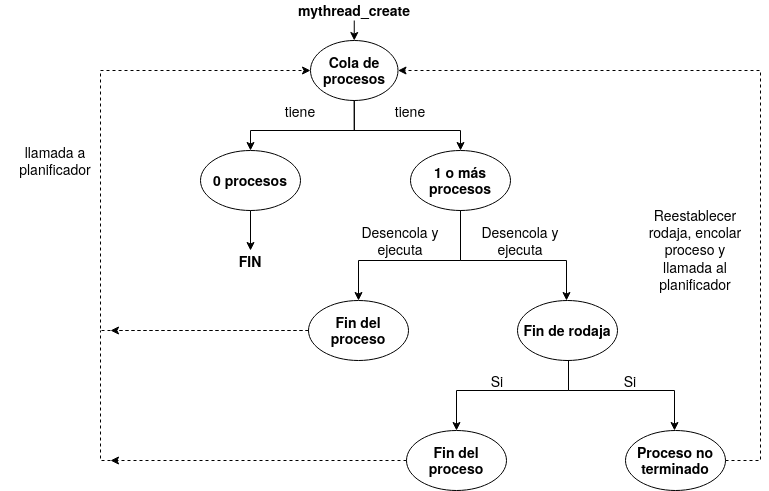
\includegraphics[width=10cm]{arboles/testRR.png}
    \caption{Árbol de pruebas Round Robin.}
    \label{fig:testRR}
\end{figure}

Como se puede ver, hay 2 opciones: que la \textbf{cola de procesos está vacía} o tenga algún proceso. En caso de estar vacía, \textbf{termina la ejecución}. Por otro lado, en caso de tener 1 o más procesos se ejecuta cada proceso el tiempo indicado en QUANTUM\_TICKS. En caso de terminar el proceso antes de finalizar dicha rodaja de tiempo, finaliza la ejecución y llamará al planificador para obtener el siguiente proceso si quedan (se implementa como \textbf{\textit{test1}}. Tabla \ref{fig:resultRR}).  

En caso de \textbf{finalizar} el tiempo marcado por cada \textbf{rodaja} pueden darse dos casos: que se haya terminado de ejecutar el hilo, a la par que termina el tiempo de la rodaja (caso implementado como \textbf{\textit{test2}}. Tabla \ref{fig:resultRR}), o que aún no haya terminado su ejecución (caso ya implementado en el \textbf{\textit{test1}}. Tabla \ref{fig:resultRR}). En el primer caso, se terminará la ejecución de dicho hilo y se procederá a \textbf{llamar al planificador para obtener el siguiente proceso si quedan}. En el segundo caso, el proceso volverá a poner el número de rodaja en su totalidad y será \textbf{encolado} en la cola de procesos, procediendo a llamar, nuevamente, al planificador.

Si llega un proceso durante la ejecución de otro proceso se encola con su rodaja correspondiente en la cola de procesos (comprobado en todos los test anteriores, principalmente en el \textbf{\textit{test1}}. Tabla \ref{fig:resultRR}).

\subsection{Round-Robin/ SJF con prioridades}
El diagrama creado para este caso ha sido el mostrado en la Figura \ref{fig:testRRS}.
\vspace{0.5cm}
\begin{figure}[h]
    \centering
    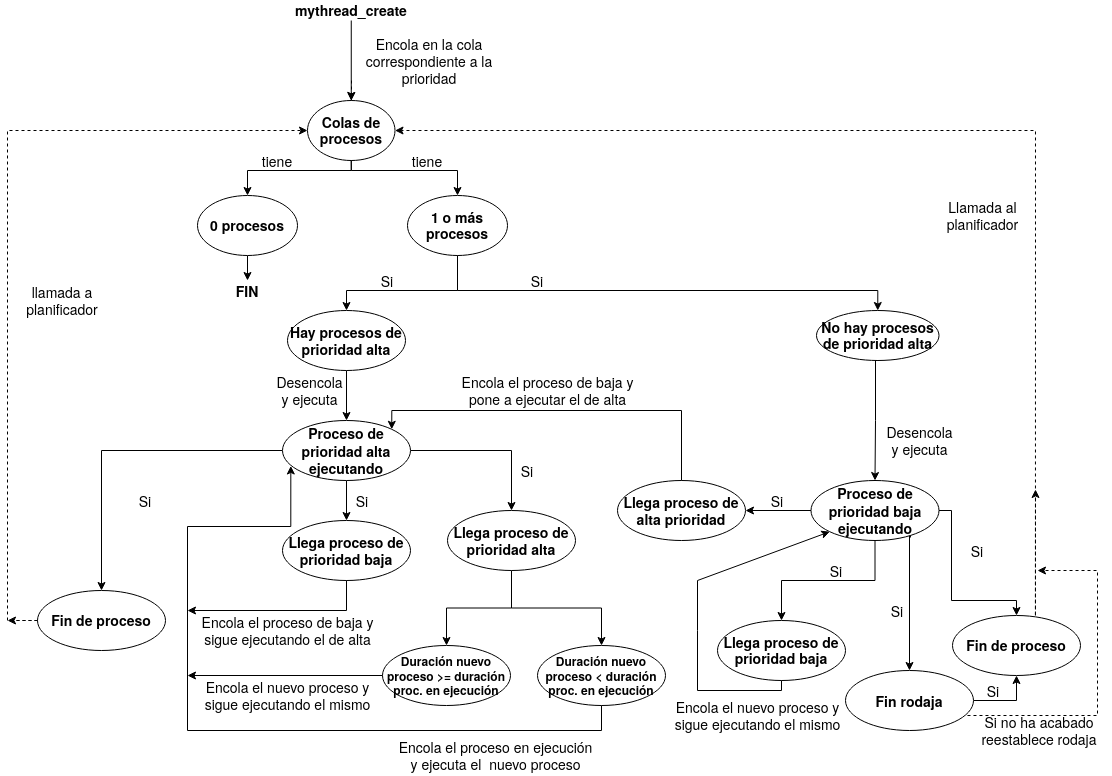
\includegraphics[width=14cm]{arboles/testRRS.png}
    \caption{Árbol de pruebas RRS}
    \label{fig:testRRS}
\end{figure}

En primer lugar, se analizan la cola de alta prioridad y la de baja prioridad, en ese orden, para ver qué proceso va a ejecutarse (llamada al planificador). En caso de no haber procesos pendientes finaliza la ejecución. En el caso de existir algún proceso pendiente, en \textbf{primer lugar} se ejecutarán aquellos procesos de \textbf{alta prioridad}. 

Si mientras se ejecuta un proceso de alta prioridad entra un proceso de \textbf{baja prioridad}, se mete este último en la cola de baja prioridad y \textbf{continúa} ejecutándose el primer proceso (caso implementado como \textbf{\textit{test3}}. Tabla \ref{fig:resultRRS}). En caso de entrar otro proceso de \textbf{alta prioridad}, sería necesario \textbf{comparar la duración} de este. Si la duración del nuevo proceso es \textbf{mayor} o igual que la duración restante del proceso en ejecución, se encola el nuevo proceso en la cola de alta prioridad y se \textbf{continúa} con la ejecución del proceso inicial (caso también comprobado en \textbf{\textit{test3}}. Tabla \ref{fig:resultRRS}). Si por el contrario la duración es menor, se realiza un cambio de contexto, por lo que el proceso que acaba de llegar pasa a ejecución y el que estaba ejecutando se encola en la cola de alta prioridad (caso implementado como \textbf{\textit{test4}}. Tabla \ref{fig:resultRRS}). Si termina la ejecución del proceso se vuelve a llamar al planificador para obtener el siguiente proceso si quedan.

Por otro lado, si al analizar ambas colas no hay procesos de alta prioridad pero sí de \textbf{baja prioridad}, pasan a ejecutarse en orden según la política \textbf{Round Robin}. En caso de encontrarse ejecutando un proceso de \textbf{baja prioridad} y entrar otro de la misma prioridad, este se \textbf{encolaría} en la cola de baja prioridad para ser ejecutado en su momento (caso implementado como \textbf{\textit{test5}}. Tabla \ref{fig:resultRRS}). Si el proceso que se está ejecutando consume el tiempo total de la rodaja, se encola reiniciando nuevamente dicho valor y se vuelven a analizar las colas. También se analiza las colas cuando el proceso en ejecución haya terminado.

Además, mientras se ejecuta un proceso de baja prioridad puede darse el caso en el que entre un proceso de \textbf{alta prioridad}. En este caso, dejará de ejecutarse el proceso actual, reiniciando la rodaja y encolándose en la cola de baja prioridad. En ese momento se \textbf{comenzaría a ejecutar} el proceso de alta prioridad (caso también implementado como \textbf{\textit{test5}}. Tabla \ref{fig:resultRRS}).



\subsection{Round-Robin/ SJF con posibles cambios de contexto voluntarios}
Para el siguiente diagrama se ha partido del diagrama adjunto en el apartado anterior. Figura \ref{fig:testRRSD}
\vspace{0.5cm}
\begin{figure}[h]
    \centering
    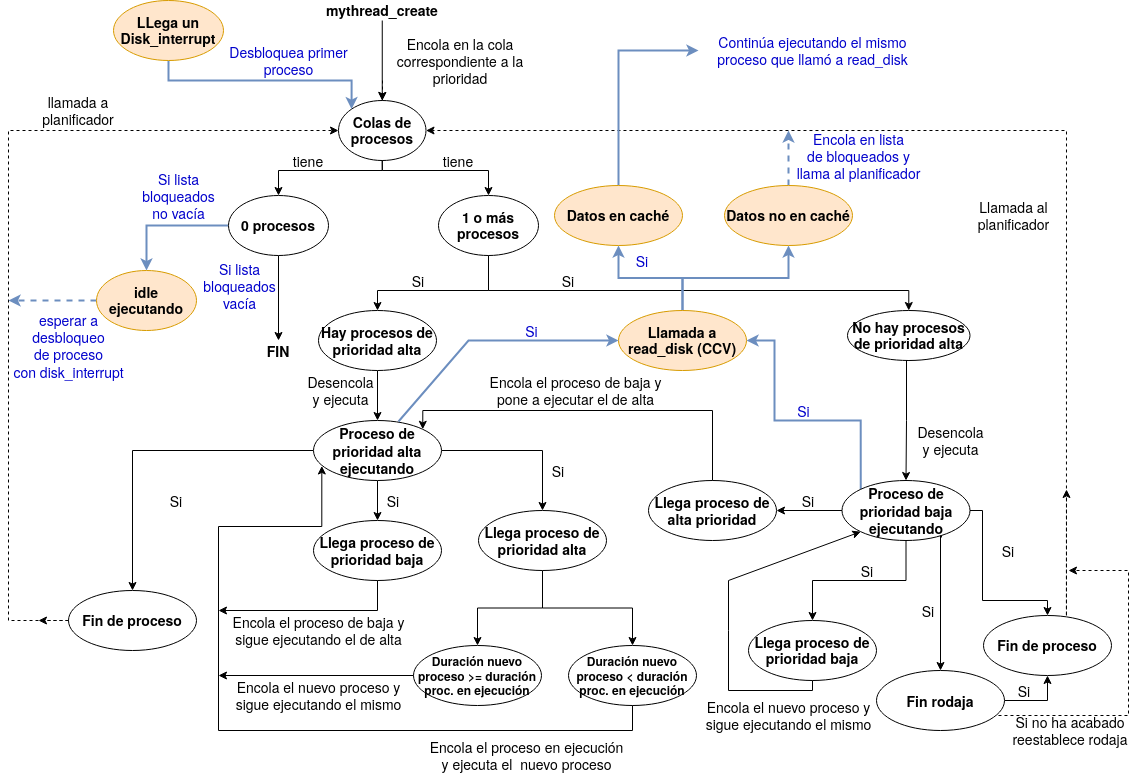
\includegraphics[width=15cm]{arboles/testRRSD.png}
    \caption{Árbol de pruebas RRSD}
    \label{fig:testRRSD}
\end{figure}

\newpage
Las diferencias se encuentran marcadas de otro color: naranja para los nodos y azul para los diversos enlaces y sus respectivos textos asociados. Como se puede apreciar, se han añadido los casos para los \textbf{cambios de contexto voluntarios} (indicados en la figura como CCV). Puesto que el código también se reutiliza, aquellas pruebas que resulten repetitivas no se han ejecutado.

Durante la ejecución de un proceso este puede requerir un cambio de contexto voluntario (llamada a \textit{read\_disk}). Si la información que requiere el proceso se encuentra \textbf{en caché}, el proceso tomará dichos datos y \textbf{continuará} su ejecución sin realizar ninguna acción más (caso implementado como \textbf{\textit{test6}} este caso vamos a probar que se realiza correctamente tanto para hilos de alta como baja prioridad. Tabla \ref{fig:resultRRSD}), dependiendo si parte de un proceso de prioridad alta o de prioridad baja). Si por el contrario la información requerida \textbf{no} se encontrase \textbf{en memoria caché}, el proceso se añadiría a la \textbf{cola de bloqueados} y se llamaría al planificador para ejecutar el siguiente proceso que toque (caso implementado como \textbf{\textit{test7}}. Tabla \ref{fig:resultRRSD}).

En caso de no haber más procesos a ejecutar en las colas de alta y baja prioridad, si la cola de bloqueados no se encuentra vacía se pondrá en ejecución el \textbf{thread \textit{idle}}. Este thread ejecutará un bucle infinito, de tal forma que el algoritmo consulte cada tick de reloj si existe algún thread listo para ejecutar, tal y como se indica en el enunciado de la práctica (caso implementado como \textbf{\textit{test8}}. Tabla \ref{fig:resultRRSD}). 
Además, observamos que existe la interrupción \textit{disk\_interrupt} que será la encargada de desbloquear los procesos de la lista de bloqueados, sacando al primero de ellos de la cola cuando se llama a la función.

\newpage
\section{Resultados batería de pruebas}
A continuación se van a presentar, en 3 tablas diferentes, las pruebas realizadas para cada uno de los apartados pedidos, presentando información como la prueba a realizar, el objetivo de la misma y el resultado obtenido. Además, habrá una cuarta tabla con pruebas comunes, cuyo resultado es el mismo en los 3 planificadores (vamos a ejecutarlas en el planificador RRSD, puesto que es el más complejo y agrupa todo lo de los dos anteriores).

\begin{table}[h!]
    \centering
    \begin{tabular}{|C{0.2\textwidth}|C{0.35\textwidth}|C{0.35\textwidth}|}
    \hline
    \hcell{Prueba} & \hcell{Objtivo de la prueba} & \hcell{Resultado} \\ \hline
    \textbf{Test9}: vamos a crear un hilo de alta prioridad y otro de baja prioridad, siendo el hilo 0 de alta prioridad & El objetivo de esta prueba es comprobar que tanto los hilos de alta como baja prioridad son expulsados si exceden el tiempo de ejecución asignados. Para ello vamos a incluir en su función un bucle for que produzca un tiempo de ejecución mayor al propuesto, por lo que deben ser expulsados. Para el caso del RR no importa la prioridad. & 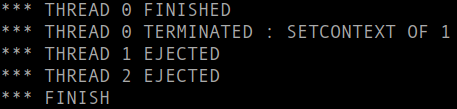
\includegraphics[width=5cm]{arboles/test9.png}
    \\ \hline
    \textbf{Test10}: el hilo 0 no va a crear ningún hilo & El objetivo es comprobar el caso en el que solo existe el hilo 0, el cual debe acabar y terminarse la ejecución & 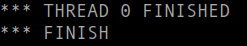
\includegraphics[width=5cm]{arboles/test10.png}. \\\hline
    \end{tabular}
    \caption{Pruebas comunes}
    \label{fig:result}
\end{table}

\begin{table}[h!]
    \centering
    \begin{tabular}{|C{0.2\textwidth}|C{0.35\textwidth}|C{0.35\textwidth}|}
    \hline
    \hcell{Prueba} & \hcell{Objtivo de la prueba} & \hcell{Resultado} \\ \hline
    \textbf{Test1}: vamos a crear hilos cuyo tiempo de ejecución sea menor a la rodaja y otros con un tiempo de ejecución mayor a la rodaja & Observar que los hilos cuyo tiempo de ejecución es inferior a la rodaja, cuando reciben el turno de ejecución, acaban su ejecución entera y realizan un exit sin llegar a hacer un swapcontext cediendo el turno (pues su rodaja aún no ha acabado), mientras que los otros hilos se irán cediendo el turno de ejecución hasta acabar. & 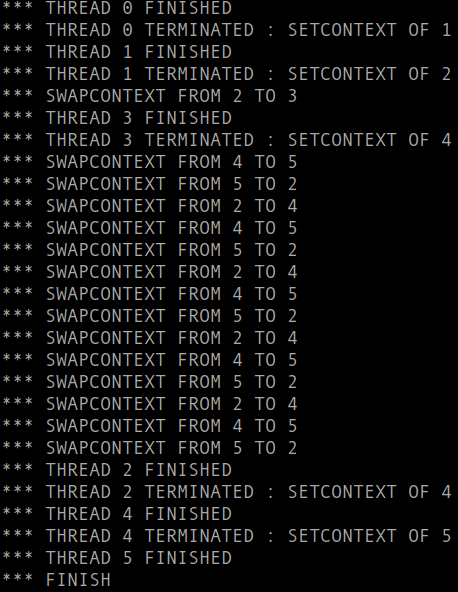
\includegraphics[width=4cm]{arboles/test1.png} \\ \hline
    \textbf{Test2}: vamos a calcular los ticks que debemos poner para que estos coincidan con el valor de la rodaja, creando un hilo con esos valores de ticks & Comprobar que ,si un hilo acaba su ejecución justo cuando la rodaja tiene valor 0, éste sale de la ejecución con un exit y no restablece su valor de rodaja y permanece en el sistema, lo cual sería un error. & 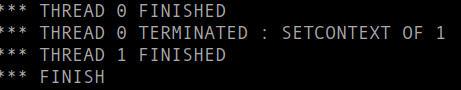
\includegraphics[width=5.5cm]{arboles/test2.png} \\\hline
    \end{tabular}
    \caption{Pruebas para RR}
    \label{fig:resultRR}
\end{table}

\newpage
\begin{table}[h!]
    \centering
    \begin{tabular}{|C{0.15\textwidth}|C{0.4\textwidth}|C{0.35\textwidth}|}
    \hline
    \hcell{Prueba} & \hcell{Objtivo de la prueba} & \hcell{Resultado} \\ \hline
    \textbf{Test3}: vamos a poner la prioridad del hilo 0 como alta. Tras esto vamos a generar algunos hilos de baja prioridad y otros de alta prioridad y cuyo tiempo de ejecución será mayor que el del main & Queremos comprobar que los hilos de baja prioridad, aunque se van a crear antes que los de alta, se ejecutarán después de estos (y respetando las rodajas). Además, crearemos 2 hilos de alta prioridad de tal manera que el último creado tendrá un menor tiempo de ejecución que el otro, comprobando que éste acaba antes pero siempre después del main, pues le hemos puesto un tiempo mayor que el del hilo 0. Esto último nos permite comprobar el caso en el que hay un hilo de prioridad alta y llega otro de prioridad alta pero con un tiempo de ejecución mayor que lo que le queda al que está ejecutando, en cuyo caso no debe cambiarse el contexto & 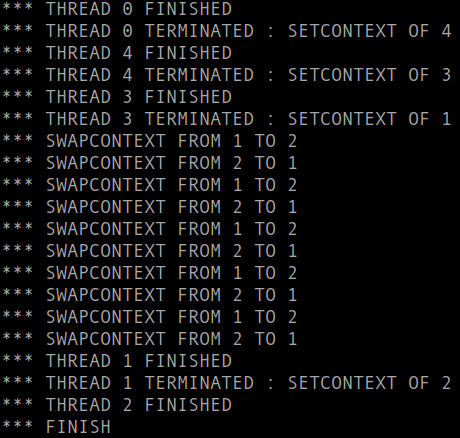
\includegraphics[width=5.9cm]{arboles/test3.png} \\ \hline
    \textbf{Test4}: vamos a poner la prioridad del hilo 0 como alta. Tras esto vamos a crear algunos hilos de prioridad alta con un tiempo de ejecución muy pequeño & El objetivo es que los hilos de alta prioridad generados tengan un tiempo de ejecución tan pequeño que sustituyan al hilo 0 en la ejecución. Así crearemos 2 hilos esperando que ambos acaben de ejecutar antes que el hilo 0. En este caso vamos a ponerles un tiempo de ejecución de 0.1 a los hilos de alta prioridad creados & 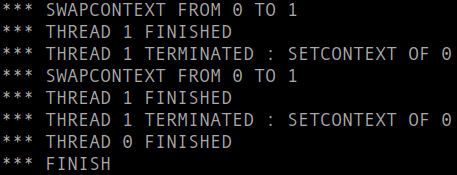
\includegraphics[width=5.5cm]{arboles/test4.png} \\\hline
    \textbf{Test5}: vamos a poner la prioridad del hilo 0 como baja. Tras esto se generarán hilos de baja prioridad y luego de alta prioridad (en ese orden) & El objetivo es observar que, si hay un hilo de prioridad baja ejecutando y llega uno de prioridad baja, los hilos se ejecutan según un RR, respetando las rodajas. Sin embargo, cuando llega uno de prioridad alta, el hilo de prioridad baja deja de ejecutar en favor del otro. Para esto generaremos varios hilos de prioridad baja en primer lugar y luego varios de prioridad alta. Debemos observar que el hilo 0 creará todos los hilos hasta llegar al primero de alta prioridad, el cuál le quitará la ejecución. Luego se ejecutarán los hilos de baja prioridad según un RR hasta crear el siguiente de prioridad alta que les quite de ejecución y así hasta acabar. & 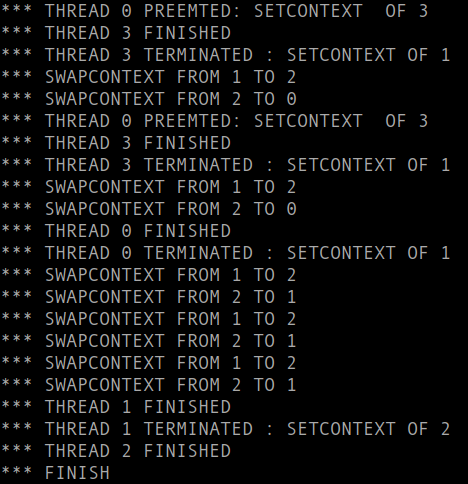
\includegraphics[width=5.9cm]{arboles/test5.png}
    \\ \hline
    \end{tabular}
    \caption{Pruebas para RRS}
    \label{fig:resultRRS}
\end{table}

\begin{table}[h!]
    \centering
    \begin{tabular}{|C{0.15\textwidth}|C{0.4\textwidth}|C{0.35\textwidth}|}
    \hline
    \hcell{Prueba} & \hcell{Objtivo de la prueba} & \hcell{Resultado} \\ \hline
    \textbf{Test6}: vamos a crear el hilo 0 de alta prioridad. Tras esto se van a crear un hilo de alta prioridad y otro de baja prioridad que van a llamar a read\_disk & Queremos comprobar cómo tanto los hilos de baja como alta prioridad, si llaman a read\_disk y obtienen que el dato está en caché, siguen con su ejecución con normalidad. Para ello vamos a incluir una llamada a read\_disk en la función de los hilos, para comprobar que ninguno de ellos se bloquea cuando los datos están en caché. El problema de esta prueba es que dependemos del dato recibido en la función data\_in\_page\_cache (si se quiere probar solo una de las prioridades es tan sencillo como comentar la creación del hilo que no se quiera) & 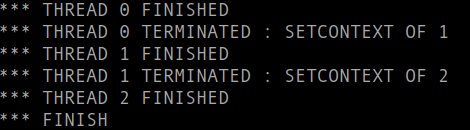
\includegraphics[width=5.5cm]{arboles/test6.png} \\ \hline
    \textbf{Test7}: vamos a crear el hilo 0 de alta prioridad. Tras esto se van a crear un hilo de alta prioridad y otro de baja prioridad que van a llamar a read\_disk & Esta prueba es exactamente igual que la anterior pero queremos observar un comportamiento distinto. En este caso queremos comprobar que los hilos de ambas prioridades, si llaman a read\_disk y los datos no están en caché, quedarán bloqueados hasta la siguiente interrupción de disco. El problema de la prueba es el mismo, se tiene que dar que ninguno de los datos esté en caché y depende de data\_in\_page\_cache & 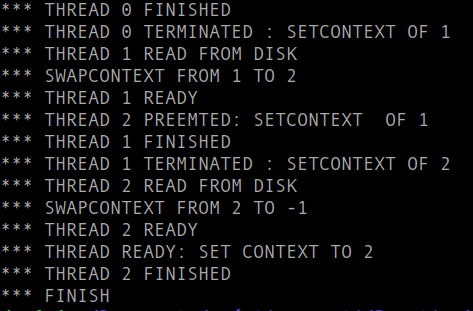
\includegraphics[width=5.5cm]{arboles/test7.png} \\\hline
    \textbf{Test8}: vamos a crear el hilo 0, con el cuál llamaremos aread\_disk & El objetivo es llamar a read\_disk con el hilo 0 y que esté se bloquee (porque los datos no están en caché). De esta forma tendremos todas las colas de procesos vacías menos la de bloqueados, por lo que el hilo idle se ejecutará hasta que el 0 se desbloquee (en pantalla se debe mostrar el cambio de contexto al hilo -1 y la impresión asociada a sacar al mismo de ejecución) & 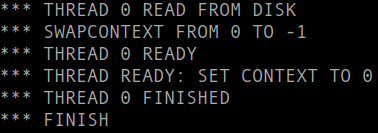
\includegraphics[width=5.5cm]{arboles/test8.png} \\\hline
   
   \end{tabular}
    \caption{Pruebas para RRSD}
    \label{fig:resultRRSD}
\end{table}

\newpage
Podemos comprobar que todas las pruebas son lo más completas posibles, evitando hacer pruebas independientes para casos muy simples que se puedan comprobar de manera conjunta en un mismo test. Así, se puede apreciar que hemos combinado ejecuciones que incluyen hilos de alta y baja prioridad cuando esto sea posible, explicando como debe ser el resultado obtenido. Además, al estar los planificadores más complejos basados en los anteriores, existen pruebas que no hemos repetido porque la ejecución es similar, como que la función mythread\_exit funcione, y nos hemos enfocado en probar las funcionalidades individuales diferenciadoras de cada planificador.

\newpage
\section{Conclusiones}
Gracias a esta práctica hemos aprendido cómo desarrollar distintos planificadores de procesos (Round-Robin, Round-Robin/SJF con prioridades y Round-Robin/SJF con cambios de contexto voluntarios), para lo que es necesario tener en cuenta, entre otras cosas, todas las estructuras de datos que necesita cada planificador (rodaja, colas de diferentes prioridades, etc.). También es necesario estudiar todos los casos posibles con detenimiento ya que, por ejemplo, no expulsar a un proceso de ejecución en su momento puede provocar errores en la ejecución que se pueden ir acumulando. 

Por otra parte, esta práctica nos ha servido para mejorar nuestra capacidades de toma de decisiones y resolución de problemas. Nos hemos tenido que enfrentar a varios dilemas como, por ejemplo, a la hora de decidir si usábamos el estado “RUNNING” para el proceso que se está ejecutando (al final hemos decidido no usarlo ya que el proceso en ejecución es el que almacena la variable “running”). Otra toma de decisión se ha dado al  debatir si era necesario usar o no la función \textit{mythread\_gettid()} para obtener el identificador de un proceso, cuando los TCB contienen un atributo que es el propio identificador del proceso al que se accede mediante “proceso.tid”.


\end{document}
